\documentclass[11pt]{article}

\usepackage[margin=1in]{geometry}
\usepackage[T1]{fontenc}
\usepackage[utf8]{inputenc}
\usepackage{lmodern}
\usepackage{microtype}
\usepackage{amsmath,amssymb}
\usepackage{booktabs}
\usepackage{graphicx}
\usepackage{subcaption}
\usepackage{enumitem}
\usepackage{array}
\usepackage{tabularx}
\usepackage{ragged2e}
\usepackage{placeins}
\usepackage{xcolor}
\usepackage{tikz}
\usepackage{pgfplots}
\usepackage[numbers]{natbib}
\usepackage[colorlinks=true,linkcolor=blue,citecolor=blue,urlcolor=blue]{hyperref}
\usepackage{xspace}

\pgfplotsset{compat=1.18}
\usetikzlibrary{positioning}
\setlength{\parskip}{0.35em}
\setlength{\parindent}{0pt}
\captionsetup{font=small,labelfont=bf}
\graphicspath{{figures/}}

\newcolumntype{Y}{>{\RaggedRight\arraybackslash}X}
\newcommand{\physiomio}{PhysioMio\xspace}

\title{Deep Neural Networks for Learning Intent from sEMG Signals to Support Hardware Devices for Post-Stroke Neurorehabilitation}
\author{
Zakariyya Brewster\\
Department of Engineering Science\\
University of Toronto
\and
Divy Wadhwani\\
Computer and Mathematical Sciences\\
University of Toronto Scarborough
\and
Emily Yan\\
Department of Computer Science\\
University of Toronto
}
\date{July 28, 2026}

\begin{document}

\maketitle

\begin{abstract}
Finger-specific motor intent is a clinically meaningful target for post-stroke neurorehabilitation, where residual muscle activity may be weak, variable, and patient-specific. This paper studies five-finger intent decoding from impaired-arm high-density surface electromyography (sEMG) using \physiomio, a bilateral longitudinal dataset collected from stroke patients~\citep{physiomioData2026}. We formulate the task as multilabel prediction and evaluate recurrent, convolutional, and graph-based decoders under a common signal-processing protocol: label alignment, 20--450 Hz Butterworth filtering, Symlet-4 wavelet denoising, 200 ms overlapping windows, and twelve handcrafted time- and frequency-domain descriptors per channel-window pair. In the direct baseline comparison, the LSTM obtains the highest subset accuracy, also called exact match ratio (0.545), while the GNN obtains the strongest macro F1 (0.706) and macro AUPRC (0.776). We then evaluate optimized CNN students and 1D ResNet teachers as deployment-oriented alternatives for Raspberry Pi 5-supported rehabilitation hardware~\citep{psrrepo2026,raspberrypi52023}. CNN-Large gives the strongest single-split aggregate CNN result, with 0.593 subset accuracy, 0.798 finger accuracy, 0.714 macro F1, 0.881 macro AUROC, and 0.812 macro AUPRC. For hardware deployment, CNN-Micro is selected because it retains similar aggregate performance at 158K parameters and an estimated 154 KB INT8 footprint. Healthy-to-impaired transfer improves the CNN-Base branch but gives mixed LSTM results. Overall, the study shows that compact neural decoders can convert post-stroke impaired-arm sEMG into five-finger intent estimates while making model-size and deployment constraints explicit.

\end{abstract}

\section{Introduction}

Finger-intent prediction from surface electromyography (sEMG) is an appealing interface for post-stroke neurorehabilitation because it offers a non-invasive path from residual muscle activity to assistive control, therapy feedback, and fine-motor retraining~\citep{munoznovoa2022upper,zheng2021semg,boukhennoufa2022wearable}. In the broader PSR project, that decoding capability is intended to support machine-learning models that can eventually be served on Raspberry Pi 5-class hardware and coupled to a rehabilitation glove. This manuscript focuses on the software research layer of that agenda: the data handling, signal processing, modeling, and evaluation work that turns multichannel sEMG into five-finger intent predictions.

The challenge is not only raw predictive accuracy, but also methodological reproducibility. Post-stroke sEMG is noisy, patient-specific, and highly sensitive to recording conditions, impairment severity, and dataset construction, so benchmark results depend heavily on how signals are filtered, denoised, segmented, labeled, tensorized, and split across patients. Reviews of sEMG-based gesture recognition consistently note that preprocessing design, feature representation, and deployment constraints can matter as much as the final classifier family~\citep{li2021gesture,ni2024survey}. A research project that reports model performance without a stable preprocessing and evaluation path is therefore difficult to audit and even harder to extend toward embedded rehabilitation use.

\repo\ addresses that gap by providing one auditable software framework for the project~\citep{psrrepo2026}. The current implementation includes \physiomio\ ingestion, gesture-to-finger label mapping, a fixed signal-conditioning stack, window-level feature extraction, shared tensor adapters, direct LSTM/CNN/GNN baselines, a merged 1D CNN student/teacher suite, Optuna-based hyperparameter optimization, healthy-to-impaired transfer-learning summaries, and benchmark artifacts stored as committed metric files. Recent project updates also added teacher-ensemble distillation, per-finger threshold tuning, and latency benchmarking utilities, which materially strengthen the edge-deployment research story even when the outputs of those utilities are not yet fully committed as benchmark bundles.

The central story of this paper is therefore research-oriented rather than repository-oriented. We do not present a new decoding architecture, nor do we claim that the current implementation already demonstrates end-to-end rehabilitation hardware validation. Instead, we report a software research program whose current contribution lies in making experimental assumptions explicit: which recordings are used, how they are preprocessed, how tensors are shared across model families, how baseline and improved architectures are compared, which metrics are computed, and which deployment-facing hooks are already present in code.

This paper makes four study-level contributions. First, it formalizes the current software pipeline from \physiomio\ ingestion through preprocessing, feature extraction, tensor adaptation, model fitting, and deployment-screening utilities. Second, it establishes a clear benchmark narrative that begins with three direct model families, LSTM, CNN, and GNN, under one preprocessing regime before analyzing subsequent improvements. Third, it evaluates two concrete improvement pathways now visible in the repository: compact CNN student and ResNet teacher development, and healthy-to-impaired transfer learning, while also documenting distillation as an implemented but not yet fully benchmarked speed-quality path. Fourth, it situates the project against the broader literature on post-stroke sEMG decoding, including PhysioMio, Ninapro, and recent transfer-learning studies, while drawing a careful boundary around what the current evidence still cannot support, especially distilled-student claims, on-device Raspberry Pi 5 validation, and clinical outcome conclusions.

\section{Related Work}

sEMG has long been studied as a non-invasive control channel for rehabilitation, prosthetics, and human-machine interaction, and stroke-specific reviews show that sEMG-driven interventions can support meaningful upper-limb rehabilitation when signal interpretation is reliable enough for assistive use~\citep{munoznovoa2022upper,zheng2021semg}. Broader reviews of wearable sensing for stroke recovery make a related point: clinical value depends on the full stack, including acquisition quality, body placement, labeling protocol, feature representation, and the way machine learning is coupled to assessment or assistive control~\citep{boukhennoufa2022wearable}. For this reason, decoding architecture should not be discussed independently of data construction and deployment context.

Dataset choice is especially important in this area. Ninapro remains the dominant public benchmark family for hand-gesture decoding from sEMG, with ten sub-datasets spanning different electrode layouts, movement vocabularies, and sensor modalities~\citep{ninapro2014,ninaproSite2026}. The widely used DB5 split, for example, records 52 movements from 10 healthy participants with two Myo armbands, while DB1 and DB2 cover larger healthy cohorts with different channel configurations and richer kinematic metadata~\citep{ninapro2014,ninaproSite2026}. By contrast, \physiomio\ was introduced in 2026 as a stroke-specific bilateral and longitudinal HD-sEMG resource with 48 stroke patients, 16 gestures, 64 electrodes, and repeated recordings across inpatient recovery~\citep{physiomioData2026}. That distinction matters because results on healthy-subject multiclass gesture sets are not automatically transferable to impaired-arm intent decoding in post-stroke populations.

Stroke-specific decoding studies have historically been small and heterogeneous. Lee et al.~\citep{lee2010stroke} used subject-specific myoelectric pattern classification for six functional hand movements in chronic stroke survivors and reported a sharp impairment-dependent gap, with mean accuracy of 71.3\% for moderately impaired participants and 37.9\% for severely impaired participants. Anastasiev et al.~\citep{anastasiev2022stroke} later studied post-acute stroke gesture recognition with portable eight-channel sEMG and found that affected-side SVM performance could still reach the high-80\% range on reduced gesture sets, but the task remained sensitive to feature design, label count, and paretic signal quality. These studies underscore a recurring challenge for post-stroke intent decoding: strong performance is possible, but dataset scale and protocol differences make general claims difficult.

Deep neural models broaden that picture but do not remove the comparability problem. Sequence-oriented recurrent models remain natural baselines because they aggregate temporal evidence across windows, while compact 1D CNNs emphasize local temporal motifs and can be compressed aggressively for efficient inference~\citep{hochreiter1997lstm}. Graph neural networks offer a complementary structural view by representing windows as related observations connected through message passing rather than as a purely linear sequence~\citep{kipf2017gcn,hamilton2017graphsage,velickovic2018gat}. On healthy-dataset benchmarks such as Ninapro, deeper end-to-end networks can reach very high multiclass accuracies; for example, Sri-Iesaranusorn et al.~\citep{sri2021dnn} reported 93.87\% accuracy on Ninapro DB5 and 91.69\% on DB7 for 41-movement classification. Those results are useful context for model capacity, but they address a different population and a different task than impaired-arm multilabel finger-intent prediction.

Transfer learning has recently become one of the most relevant directions for rehabilitation-oriented sEMG. Li et al.~\citep{li2025transfer} showed that transfer-based CNNs can materially improve inter-subject and inter-day robustness on high-density healthy-subject sEMG, and Mohammadiazni et al.~\citep{mohammadiazni2026transfer} demonstrated an especially important stroke-specific result: pretraining on healthy Ninapro DB5 data raised stroke-survivor gesture-classification accuracy from 46\% to 93.6\% in a three-gesture setting. These findings motivate the healthy-to-impaired transfer pathway in \repo, but they also raise a cautionary point. Transfer-learning gains are task-, architecture-, and dataset-dependent, so a project paper should report them as empirical outcomes rather than as guaranteed improvements.

Deployment-oriented optimization provides the final piece of context for this manuscript. Knowledge distillation is a standard way to transfer behavior from larger teachers into smaller students~\citep{hinton2015distilling}, and Optuna is widely used for black-box hyperparameter search under practical constraints~\citep{akiba2019optuna}. What distinguishes \repo\ is therefore not a novel recurrent, convolutional, or graph formulation in isolation, but an integrated software research effort that places dataset harmonization, baseline comparison, teacher-student modeling, transfer learning, and deployment proxies inside one auditable experimental framework.

\begin{table}[t]
  \centering
  \footnotesize
  \caption{Literature context used to position the current study. Reported numbers come from different populations, sensors, gesture vocabularies, and label spaces, so the table is for context rather than for a direct leaderboard comparison.}
  \label{tab:literature-context}
  \resizebox{\linewidth}{!}{\begin{tabularx}{\linewidth}{>{\RaggedRight\arraybackslash}p{2.15cm}YYYY}
\toprule
Source & Population / dataset & Task & Reported performance & Relevance to this paper \\
\midrule
Lee et al. 2010 & 20 chronic stroke survivors; 10 forearm/hand electrodes & Six functional hand movements with subject-specific EMG classification & Mean accuracy 71.3\% for moderate impairment and 37.9\% for severe impairment & Early evidence that stroke severity strongly affects decoder quality \\
Anastasiev et al. 2022 & 19 post-acute stroke patients; portable eight-channel sEMG & Four- to seven-gesture multiclass recognition on affected and non-affected sides & Affected-side SVM accuracy reached 88.7\% on the four-gesture setting & Shows that reduced-vocabulary stroke gesture recognition can reach high accuracy with careful feature design \\
Bao et al. 2024 & 8 chronic stroke participants; post-stroke sEMG feature-domain study & CNN, CNN-LSTM, and CNN-LSTM-attention recognition using time, frequency, and wavelet features & Best reported averages: 72.95\% intra-subject accuracy and 68.38\% inter-subject transfer accuracy & Supports deep architectures for post-stroke decoding while highlighting the difficulty of transfer \\
\parbox[t]{2.15cm}{Mohammadiazni\\et al. 2026} & 10 stroke patients plus healthy Ninapro DB5 pretraining data & Three-gesture classification across multiple arm postures with transfer learning & 93.6\% with transfer learning versus 46\% without transfer & Strong stroke-specific motivation for healthy-to-impaired transfer learning \\
\parbox[t]{2.15cm}{Sri-Iesaranusorn\\et al. 2021} & Ninapro DB5/DB7, mostly healthy-subject settings & 41-movement deep neural network classification & 93.87\% on DB5 and 91.69\% on DB7 & Healthy-data ceiling is high, but the task is easier than impaired-arm multilabel finger decoding \\
This project & \physiomio\ impaired-arm split from 48 stroke patients; patient-level train/val/test split & Five-finger multilabel intent decoding and four-channel hardware-targeted retraining & CNN-Large: 0.593 subset accuracy and 0.714 macro F1; distilled four-channel CNN-Micro: $0.522\pm0.011$ and $0.609\pm0.006$ & Connects impaired-arm model comparison to a concrete reduced-sensor interface \\
\bottomrule
\end{tabularx}
}
\end{table}

\section{Method}

\subsection{Overview}

This project defines a modular decoding workflow from multichannel sEMG and gesture annotations to five-finger prediction logits. The pipeline contains four stages: data harmonization, signal processing, model inference, and evaluation or deployment analysis. Figure~\ref{fig:pipeline} summarizes the workflow used throughout the study.

\begin{figure}[t]
  \centering
  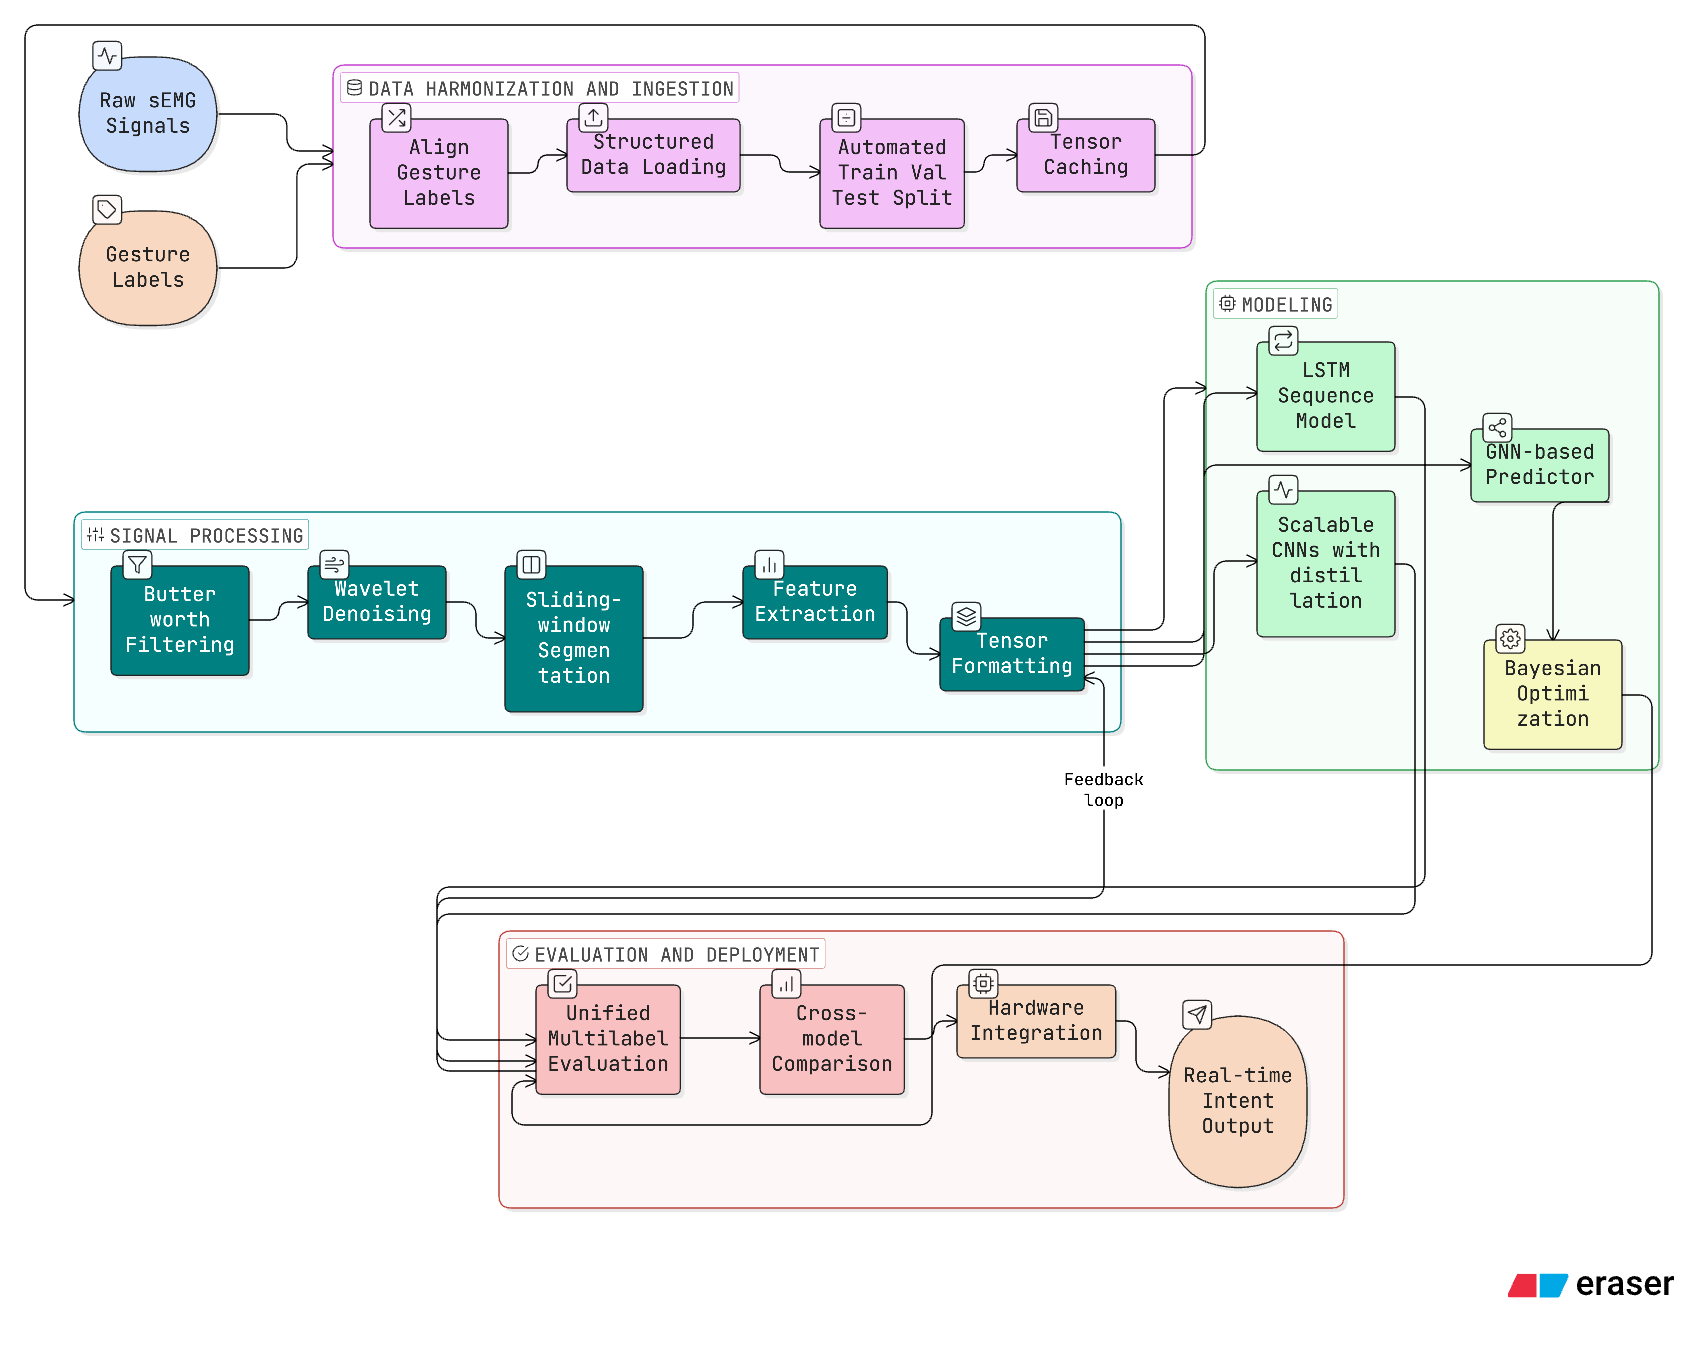
\includegraphics[width=\linewidth,trim=35 120 35 70,clip]{pipeline_overview.png}
  \caption{Overview of the sEMG finger-intent decoding pipeline. Raw sEMG and gesture annotations are aligned, segmented, featurized, mapped into shared tensors, evaluated across multiple model families, and prepared for downstream deployment analysis.}
  \label{fig:pipeline}
\end{figure}

For notation, let a pre-segmented recording be $X \in \mathbb{R}^{T \times C}$, where $T$ is the number of raw time samples and $C=64$ is the channel count under the \physiomio\ path. After preprocessing and windowing, the project extracts a feature tensor $\mathcal{X} \in \mathbb{R}^{C \times W \times F}$, where $W$ is the number of windows and $F=12$ is the number of handcrafted descriptors per channel-window pair. Each sample is paired with a multilabel target vector $y \in \{0,1\}^5$ indicating intended activation of thumb, index, middle, ring, and little finger.

\subsection{Data harmonization and ingestion}

The implementation builds processed datasets directly from raw \physiomio\ parquet files. The loader searches the raw data tree, groups files by patient, aligns contiguous stretches of the same \texttt{movement\_type}, maps each label to a five-bit finger target, discards segments shorter than 200 samples, and applies the preprocessing pipeline to each usable segment. This converts gesture-level clinical recordings into segment-level multilabel examples.

The default configuration uses \physiomio\ recordings sampled at 2000 Hz and selects the impaired arm. Patients are partitioned into deterministic 70/10/20 train/validation/test splits, so samples from the same patient do not appear in multiple partitions. Processed samples are padded to a dataset-wide maximum window count for batched tensor operations.

\subsection{Signal preprocessing}

The preprocessing module is explicitly parameterized by a frozen configuration object in the implementation. Raw sEMG first passes through a fourth-order Butterworth band-pass filter with 20--450 Hz cutoffs and zero-phase forward-backward application. This stage suppresses low-frequency motion artifacts and high-frequency electrical noise while preserving time alignment across channels.

The filtered signal is then denoised with wavelet soft-thresholding. The default configuration uses a Symlet-4 basis, four decomposition levels, universal threshold selection, and a median-based noise estimate. The same preprocessing configuration is used for all model families, making downstream differences attributable to the representation and predictor rather than to separate signal-conditioning choices.

After denoising, each continuous segment is divided into 200 ms windows with 50\% overlap and no zero-padding. These settings balance temporal responsiveness against the sample count required for stable summary statistics.

\subsection{Window-level feature representation}

Each channel-window pair is summarized by twelve handcrafted descriptors spanning time and frequency domains. The time-domain set includes root mean square, mean absolute value, integrated EMG, waveform length, variance, zero crossings, slope sign changes, and Willison amplitude. The frequency-domain set includes mean frequency, median frequency, spectral entropy, and total power, with spectral quantities estimated from Welch periodograms using \texttt{nperseg = min(256, len(x))}~\citep{welch1967fft}. Degenerate spectra are zeroed explicitly to avoid unstable feature values. The resulting tensor has shape $(C, W, F)$, where $C$ is the number of channels, $W$ is the number of windows, and $F=12$ is the feature count.

\subsection{Tensor formatting and shared adapter}

The project standardizes cross-model comparison with one shared adapter. It transforms $(C, W, F)$ or $(N, C, W, F)$ tensors into $(N, W, C \times F)$ sequences, where windows act as time steps and all channel features are concatenated into one vector per step. For a single sample, the adapted sequence can be written as
\[
S = \left[s_1, \ldots, s_W\right]^\top \in \mathbb{R}^{W \times d},
\qquad
s_w = \mathrm{vec}\!\left(\mathcal{X}_{:,w,:}\right),
\qquad
d = C F = 768.
\]
This adapter creates a common input space for recurrent, convolutional, and graph-based predictors.

For the CNN branch, the adapted tensor is subsequently permuted to a channels-first layout. The CNN stack treats the $64 \times 12$ channel-feature grid as 768 input channels for temporal \texttt{Conv1d} layers, preserving the same upstream representation while allowing convolutions over window order.

\subsection{Predictor families}

The LSTM branch applies two stacked recurrent layers with hidden sizes 128 and 256, followed by a 128-unit fully connected layer and dropout before five output logits. Given adapted sequence input $s_t$, the recurrent dynamics follow the standard LSTM update
\[
\begin{aligned}
i_t &= \sigma(W_i s_t + U_i h_{t-1} + b_i), \\
f_t &= \sigma(W_f s_t + U_f h_{t-1} + b_f), \\
o_t &= \sigma(W_o s_t + U_o h_{t-1} + b_o), \\
\tilde{c}_t &= \tanh(W_c s_t + U_c h_{t-1} + b_c), \\
c_t &= f_t \odot c_{t-1} + i_t \odot \tilde{c}_t, \\
h_t &= o_t \odot \tanh(c_t),
\end{aligned}
\]
and the project uses the final hidden state from the second recurrent layer for classification. This branch emphasizes temporal accumulation across windows and serves as the main sequential baseline for the direct benchmark.

The GNN branch interprets each time window as a node in a graph. The implementation supports GCN, GraphSAGE, and GAT operators~\citep{kipf2017gcn,hamilton2017graphsage,velickovic2018gat}, and the benchmarked path constructs a dense graph over windows within each sample before graph-level pooling and readout. At a generic level, the node update can be written as
\[
h_i^{(\ell+1)} =
\psi_\ell\!\left(
h_i^{(\ell)},
\operatorname*{AGG}_{j \in \mathcal{N}(i)}
\phi_\ell\!\left(h_i^{(\ell)}, h_j^{(\ell)}\right)
\right),
\]
followed by graph pooling
\[
g = \operatorname*{POOL}_{i=1}^{W} h_i^{(L)}
\]
and a multilabel readout head. This branch injects an explicit structural prior: windows are related observations rather than only a flat sequence.

The CNN branch includes five student variants ranging from Nano to XLarge, each built around a $1 \times 1$ projection, temporal convolution blocks, adaptive pooling, and a compact fully connected head. If the channels-first representation is denoted by $\hat{S} \in \mathbb{R}^{d \times W}$, the student stack can be summarized as
\[
H^{(0)} = \rho\!\left(\operatorname{BN}(W_p * \hat{S} + b_p)\right),
\qquad
H^{(\ell+1)} = \rho\!\left(\operatorname{BN}(W_\ell * H^{(\ell)} + b_\ell)\right),
\]
where $*$ denotes 1D convolution over window order and $\rho$ is a ReLU nonlinearity. Adaptive pooling compresses the temporal axis before a multilayer perceptron produces the five logits. The student family spans approximately 54K parameters and 53 KB INT8 for Nano to 1.62M parameters and 1.58 MB INT8 for XLarge. The teacher family uses 1D ResNet-50, ResNet-101, and ResNet-152 variants with bottleneck residual blocks.

\subsection{Training, tuning, and evaluation protocol}

The training utilities unify optimization and reporting across model families. The current implementation uses binary cross-entropy with logits for five-label prediction, Adam-based optimization, plateau-triggered learning-rate reduction, early stopping, checkpointing, and saved metric curves. For logits $z \in \mathbb{R}^5$, the base multilabel objective is
\[
\mathcal{L}_{\mathrm{BCE}}
=
-\frac{1}{5}
\sum_{k=1}^{5}
\left[
y_k \log \sigma(z_k)
+ (1-y_k) \log \left(1-\sigma(z_k)\right)
\right].
\]
Evaluation reports exact-match accuracy, finger-level averaged accuracy, macro precision, macro recall, macro F1, macro AUROC, and macro AUPRC. The metrics module also stores per-finger scores and task-level curve data, which enables both aggregate and finger-wise analysis after training.

For the CNN students, Optuna searches architecture and training choices for each model size, and the optimization score combines validation accuracy with a latency-based penalty relative to a baseline timing reference~\citep{akiba2019optuna}. Trial-level early stopping is used during search. The system also supports teacher-ensemble distillation, per-finger threshold tuning, and latency benchmarking. For multilabel distillation, the implemented loss blends the hard target term with a temperature-scaled soft target from the teacher,
\[
\mathcal{L}_{\mathrm{KD}}
=
\alpha \, \mathcal{L}_{\mathrm{BCE}}(z_s, y)
+
(1-\alpha) T^2
\operatorname{BCELogits}\!\left(\frac{z_s}{T}, \sigma\!\left(\frac{z_t}{T}\right)\right),
\]
where $z_s$ and $z_t$ are student and teacher logits, $T$ is the distillation temperature, and $\alpha$ controls the hard-soft balance. A separate latency benchmark reports mean, median, and 95th-percentile inference time on a chosen device.

\subsection{Transfer-learning path}

In addition to direct impaired-arm benchmarks, the study evaluates two-stage CNN and LSTM training. Models are first pretrained on healthy-arm recordings and then finetuned on impaired-arm recordings while preserving the same five-finger multilabel objective. This tests whether healthy-limb structure can provide a useful initialization for paretic-limb decoding.

\section{Experiments}

\subsection{Dataset and split construction}

All experiments use the \physiomio\ processing path implemented for this project~\citep{physiomioData2026,psrrepo2026}. The dataset construction step extracts contiguous movement segments from raw parquet recordings, maps gesture labels to five-bit finger targets, preprocesses each segment, and stores processed tensors as PyTorch split files.

Patients are shuffled with a fixed seed and divided into 70\% train, 10\% validation, and 20\% test partitions. The main benchmark uses impaired-arm recordings. The transfer-learning experiments use healthy-arm recordings for pretraining and impaired-arm recordings for finetuning.

\subsection{Model groups}

The experiments are organized into three groups. The first group compares direct LSTM, CNN, and GNN baselines trained under the same preprocessing and feature representation. The second group evaluates optimized CNN students and ResNet teachers, emphasizing the trade-off between multilabel performance and model footprint. The third group evaluates healthy-to-impaired transfer learning. Distillation is implemented in the codebase as a teacher-student compression path, but it is not reported as a completed benchmark in the current results.

\subsection{Evaluation protocol}

The task is five-label multilabel classification with a nominal decision threshold of 0.5 on the held-out test split. We report subset accuracy, also called exact match ratio, mean finger accuracy, macro precision, macro recall, macro F1, macro AUROC, macro AUPRC, and per-finger metrics. Subset accuracy is strict because all five labels must be correct for a sample to count as correct; finger accuracy and macro metrics expose behavior that subset accuracy alone can hide. The present tables report single deterministic train/validation/test split estimates from committed artifacts, so small differences should be interpreted as empirical comparisons rather than statistical significance claims.

The Results section follows the experimental sequence: direct baselines, optimized CNN students and ResNet teachers, transfer learning, finger-level behavior, and literature positioning.

\section{Results}

\subsection{Direct baseline models: LSTM, CNN, and GNN}

The first layer of evidence is the direct three-family comparison that motivated the project before later CNN refinements were merged. Table~\ref{tab:model-comparison} shows the held-out impaired-arm metrics for the original LSTM, CNN, and GNN runs under the shared preprocessing path. No single family dominates every metric. The LSTM is the strongest baseline on exact-match accuracy and macro AUROC, the GNN is best on macro F1 and macro AUPRC, and the legacy CNN is competitive on finger accuracy but otherwise trails the other two branches.

\begin{table}[t]
  \centering
  \small
  \caption{Held-out test performance for the three direct model families. Bold numbers mark the best score in each column within this baseline comparison only.}
  \label{tab:model-comparison}
  \begin{tabular}{lccccc}
\toprule
Model & Subset Acc. & Finger Acc. & Macro F1 & Macro AUROC & Macro AUPRC \\
\midrule
LSTM & \textbf{0.545} & \textbf{0.784} & 0.705 & \textbf{0.858} & 0.754 \\
CNN legacy & 0.442 & 0.694 & 0.676 & 0.767 & 0.764 \\
GNN  & 0.448 & 0.683 & \textbf{0.706} & 0.787 & \textbf{0.776} \\
\bottomrule
\end{tabular}

\end{table}

\begin{figure}[t]
  \centering
  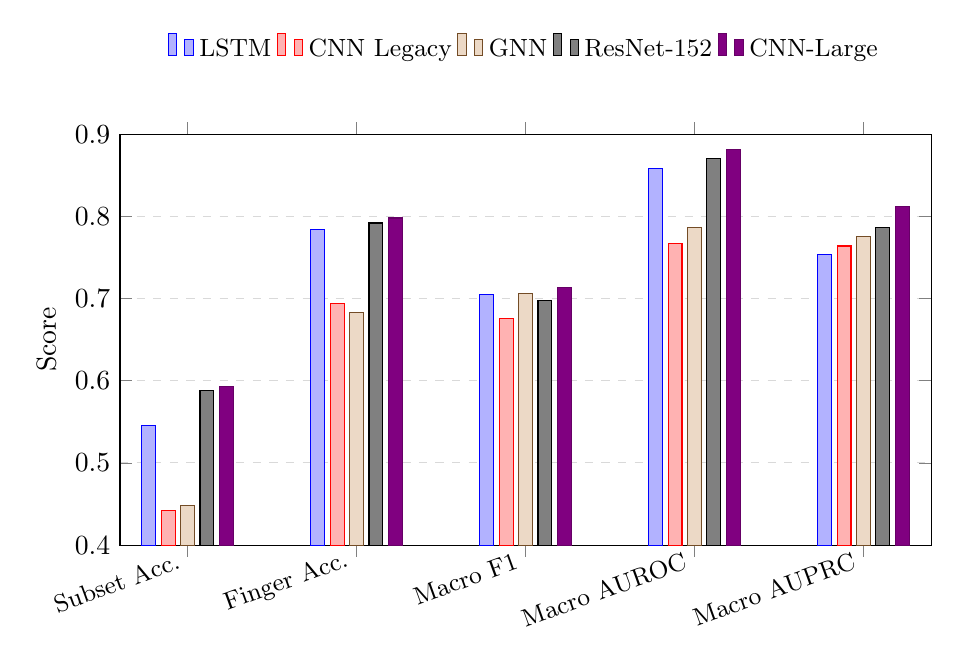
\begin{tikzpicture}
\begin{axis}[
  ybar,
  width=0.98\linewidth,
  height=6.8cm,
  ymin=0.40,
  ymax=0.90,
  ylabel={Score},
  symbolic x coords={Subset Acc.,Finger Acc.,Macro F1,Macro AUROC,Macro AUPRC},
  xtick=data,
  xticklabel style={rotate=20,anchor=east,font=\small},
  ymajorgrids=true,
  grid style={dashed,gray!30},
  legend style={at={(0.5,1.15)},anchor=south,legend columns=-1,draw=none,font=\small},
  bar width=5pt,
]
\addplot coordinates {(Subset Acc.,0.545) (Finger Acc.,0.784) (Macro F1,0.705) (Macro AUROC,0.858) (Macro AUPRC,0.754)};
\addplot coordinates {(Subset Acc.,0.442) (Finger Acc.,0.694) (Macro F1,0.676) (Macro AUROC,0.767) (Macro AUPRC,0.764)};
\addplot coordinates {(Subset Acc.,0.448) (Finger Acc.,0.683) (Macro F1,0.706) (Macro AUROC,0.787) (Macro AUPRC,0.776)};
\addplot coordinates {(Subset Acc.,0.588) (Finger Acc.,0.792) (Macro F1,0.698) (Macro AUROC,0.870) (Macro AUPRC,0.787)};
\addplot coordinates {(Subset Acc.,0.593) (Finger Acc.,0.798) (Macro F1,0.714) (Macro AUROC,0.881) (Macro AUPRC,0.812)};
\legend{LSTM,CNN Legacy,GNN,ResNet-152,CNN-Large}
\end{axis}
\end{tikzpicture}

  \caption{Aggregate-metric comparison across the three direct baselines plus the strongest internal teacher and student references from the newer CNN branch.}
  \label{fig:model-comparison}
\end{figure}

This baseline table is important because it supports the paper's first claim: the project did not begin as a single-model CNN paper. It began as a cross-family study in which recurrent, graph, and convolutional views of the same feature representation each offered different trade-offs. That observation still matters after the newer CNN work is added, because it explains why the repository contains multiple model families and why finger-level analysis remains useful even when one branch improves the aggregate scores.

\subsection{Performance-improvement path: optimized CNN students and ResNet teachers}

The second layer of evidence asks whether the repository's newer CNN branch materially shifts the benchmark frontier. Table~\ref{tab:cnn-sweep} answers yes. Relative to the legacy CNN baseline, the optimized student family improves all major aggregate metrics, and the strongest student, CNN-Large, becomes the best committed model artifact in the repository with 0.593 exact-match accuracy, 0.798 finger accuracy, 0.714 macro F1, 0.881 macro AUROC, and 0.812 macro AUPRC.

\begin{table}[t]
  \centering
  \small
  \caption{Detailed CNN-family evaluation. Student parameter counts and INT8 sizes come from the project CNN README; teacher rows are included as internal high-capacity reference models merged through PR~56. Bold numbers mark the best score in each column across the rows shown.}
  \label{tab:cnn-sweep}
  \resizebox{\linewidth}{!}{\begin{tabular}{llccccccc}
\toprule
Variant & Type & Params & INT8 Size & Subset Acc. & Finger Acc. & Macro F1 & Macro AUROC & Macro AUPRC \\
\midrule
ResNet-50  & Teacher & --    & --      & 0.570 & 0.788 & 0.656 & 0.840 & 0.772 \\
ResNet-101 & Teacher & --    & --      & 0.569 & 0.795 & 0.681 & 0.852 & 0.767 \\
ResNet-152 & Teacher & --    & --      & 0.588 & 0.792 & 0.698 & 0.870 & 0.787 \\
\midrule
Nano        & Student & 54K   & 53 KB   & 0.580 & 0.794 & 0.698 & 0.855 & 0.758 \\
Micro$^\dagger$ & Student & 158K  & 154 KB  & 0.578 & 0.794 & 0.697 & 0.871 & 0.793 \\
Base        & Student & 390K  & 381 KB  & 0.575 & \textbf{0.798} & 0.707 & 0.870 & 0.775 \\
Large       & Student & 803K  & 784 KB  & \textbf{0.593} & \textbf{0.798} & \textbf{0.714} & \textbf{0.881} & \textbf{0.812} \\
XLarge      & Student & 1.62M & 1.58 MB & 0.551 & 0.794 & 0.690 & 0.830 & 0.726 \\
\bottomrule
\end{tabular}
}
\end{table}

Several observations follow from Table~\ref{tab:cnn-sweep}. First, the change from the legacy CNN to the optimized CNN-Large artifact is substantial rather than cosmetic: exact-match accuracy rises from 0.442 to 0.593, macro F1 from 0.676 to 0.714, macro AUROC from 0.767 to 0.881, and macro AUPRC from 0.764 to 0.812. Second, the compact Nano and Micro students remain close to the larger models despite much smaller INT8 footprints, which is the clearest current evidence for the project's edge-oriented design goal. Third, the teacher results provide a meaningful internal reference. Among the committed teacher checkpoints, ResNet-152 is the strongest teacher with 0.588 exact-match accuracy and 0.698 macro F1, yet CNN-Large still slightly exceeds it on exact-match accuracy, macro F1, macro AUROC, and macro AUPRC. This does not prove that distillation is already responsible for the gain, because the repository does not yet commit a comparable distilled-student result set. It does show that the tuned student branch is already competitive with its larger teacher family.

\subsection{Improvement paths for metrics and speed}

Transfer-learning summaries in Table~\ref{tab:transfer-learning} show a deliberately asymmetric result: one path works clearly, one does not. For the CNN branch, healthy-to-impaired staging improves exact-match accuracy from 0.465 to 0.585 and finger accuracy from 0.760 to 0.800 while also improving macro AUROC and macro AUPRC. For the LSTM branch, finetuning improves exact-match and finger accuracy but lowers macro F1, macro AUROC, and macro AUPRC relative to the healthy pretraining summary. The practical conclusion is that healthy-arm pretraining is already a credible improvement path for the CNN family in this repository, but not a universally beneficial recipe across architectures.

\begin{table}[t]
  \centering
  \small
  \caption{Committed healthy-to-impaired transfer-learning summaries. The CNN branch benefits consistently after finetuning; the LSTM branch improves on exact-match and finger accuracy but loses ground on ranking-sensitive metrics.}
  \label{tab:transfer-learning}
  \begin{tabular}{lccccc}
\toprule
Model / Stage & Exact-match & Finger Acc. & Macro F1 & Macro AUROC & Macro AUPRC \\
\midrule
CNN pre. & 0.465 & 0.760 & 0.664 & 0.833 & 0.699 \\
CNN fine. & \textbf{0.585} & \textbf{0.800} & \textbf{0.680} & \textbf{0.863} & \textbf{0.767} \\
LSTM pre. & 0.523 & 0.752 & \textbf{0.679} & \textbf{0.858} & \textbf{0.773} \\
LSTM fine. & \textbf{0.574} & \textbf{0.777} & 0.660 & 0.830 & 0.736 \\
\bottomrule
\end{tabular}

\end{table}

Distillation is best interpreted differently. The repository now contains teacher-ensemble distillation code, explicit multilabel distillation losses, threshold-tuning utilities, and latency-benchmarking scripts, all of which are aligned with the project's goal of improving the speed-quality trade-off for Raspberry Pi-class deployment. However, the current artifact set still lacks a mature distilled-student evaluation bundle and committed on-device timing logs. The distillation story is therefore architectural and procedural rather than empirical at this stage: it is an implemented path for future speed and compression gains, not yet a closed result in the same sense as the direct or transfer tables.

\subsection{Finger-level behavior and external positioning}

Finger-wise scores show that the ranking is not uniform across all outputs. Table~\ref{tab:per-finger-f1} compares the LSTM direct baseline, the GNN direct baseline, and the best optimized CNN student. The GNN remains strongest on the thumb label, the optimized CNN-Large leads on index and little finger, and the LSTM remains slightly strongest on middle and ring finger. This pattern suggests that aggregate CNN gains do not erase all output-specific variation; different inductive biases still matter at the finger level.

\begin{table}[t]
  \centering
  \small
  \caption{Per-finger F1 score by model family. The optimized CNN-Large replaces the legacy direct CNN row for the finger-level comparison. Bold numbers mark the strongest model for each finger.}
  \label{tab:per-finger-f1}
  \begin{tabular}{lccc}
\toprule
Finger & LSTM & GNN & CNN \\
\midrule
Thumb  & 0.716 & \textbf{0.776} & 0.726 \\
Index  & \textbf{0.723} & 0.696 & 0.660 \\
Middle & \textbf{0.712} & 0.689 & 0.675 \\
Ring   & \textbf{0.696} & 0.688 & 0.670 \\
Little & \textbf{0.680} & 0.678 & 0.649 \\
\bottomrule
\end{tabular}

\end{table}

\begin{figure}[t]
  \centering
  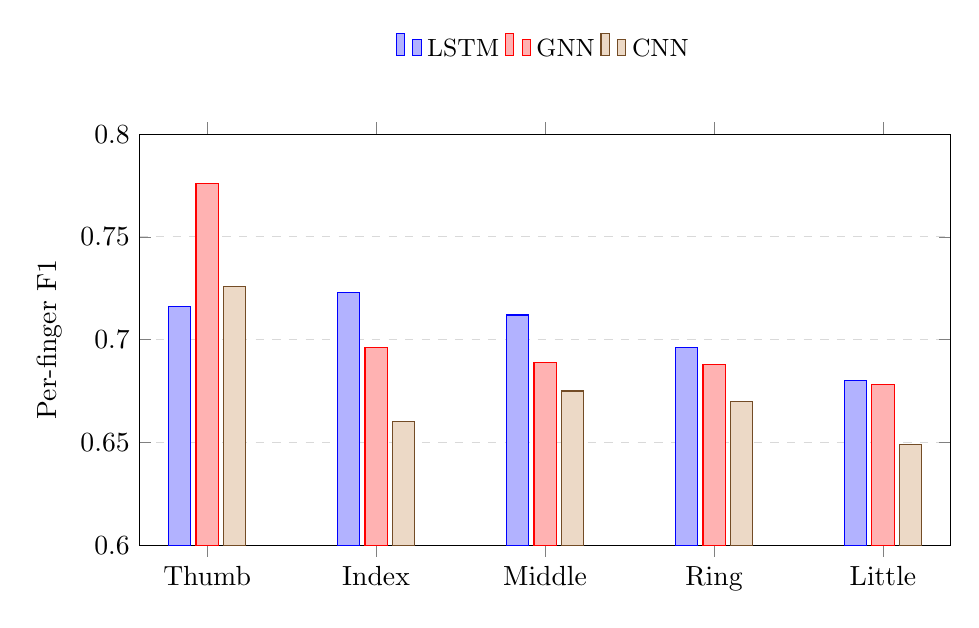
\begin{tikzpicture}
\begin{axis}[
  ybar,
  width=0.98\linewidth,
  height=6.8cm,
  ymin=0.60,
  ymax=0.80,
  ylabel={Per-finger F1},
  symbolic x coords={Thumb,Index,Middle,Ring,Little},
  xtick=data,
  ymajorgrids=true,
  grid style={dashed,gray!30},
  legend style={at={(0.5,1.15)},anchor=south,legend columns=-1,draw=none,font=\small},
  bar width=8pt,
]
\addplot coordinates {(Thumb,0.716) (Index,0.723) (Middle,0.712) (Ring,0.696) (Little,0.680)};
\addplot coordinates {(Thumb,0.776) (Index,0.696) (Middle,0.689) (Ring,0.688) (Little,0.678)};
\addplot coordinates {(Thumb,0.726) (Index,0.660) (Middle,0.675) (Ring,0.670) (Little,0.649)};
\legend{LSTM,GNN,CNN}
\end{axis}
\end{tikzpicture}

  \caption{Per-finger F1 comparison derived from the committed metric files. Aggregate CNN gains coexist with output-specific strengths for the LSTM and GNN baselines.}
  \label{fig:per-finger-f1}
\end{figure}

To show where this project stands relative to the literature, Table~\ref{tab:literature-context} should be read alongside the internal results rather than against them. Prior stroke-decoding papers often report much higher accuracies than our exact-match scores, but they typically solve easier multiclass tasks with fewer gestures, fewer labels, smaller cohorts, or healthy-data pretraining. Our current numbers are stricter in at least three ways: they use a five-finger multilabel formulation, they are derived from impaired-arm \physiomio\ recordings with patient-level splits, and the headline exact-match metric requires all five finger labels to be correct simultaneously. For that reason, the more meaningful external takeaway is not that \repo\ already leads the literature, but that it now occupies a technically credible position: stronger than a simple proof-of-concept, richer than a single-model benchmark, and explicit enough to support future work on transfer, distillation, and embedded deployment.

The results should nevertheless be read with an evidence boundary in mind. The project now includes code for teacher-ensemble distillation, per-finger threshold tuning, and CPU latency measurement, but it does not yet commit a mature result bundle produced by those new utilities, nor does it store on-device Raspberry Pi 5 timings. The current paper can therefore support a stronger research narrative than the previous draft, but not a full claim of embedded deployment readiness.

\section{Discussion}

The results support three main observations about post-stroke finger-intent decoding from HD-sEMG. First, no single inductive bias is uniformly superior in the direct baseline setting. The LSTM's advantage on subset accuracy suggests that recurrent state can help produce coherent multi-finger predictions across a segment, while the GNN's macro F1 and AUPRC indicate strong class-balanced discrimination when windows are modeled as related observations. This is consistent with the structure of the task: paretic sEMG contains both temporal continuity and non-local relationships among windows.

Second, the optimized CNN results show that compact temporal convolution can be effective once the architecture is tuned for the feature representation. The direct CNN baseline is weak, but the tuned student sweep shows that this is not a limitation of temporal convolution as a model family. CNN-Large gives the strongest offline aggregate CNN result in the current single-split experiments, but CNN-Micro is the deployment model chosen for the Raspberry Pi 5 pathway because it keeps the accuracy and ranking metrics close to CNN-Large while reducing the estimated INT8 footprint from 784 KB to 154 KB. The poorer CNN-XLarge result reinforces the same point from the opposite direction: increasing capacity alone is not enough, and the useful operating point is determined by the interaction among data scale, regularization, search budget, and deployment constraints.

Third, transfer learning appears useful but architecture-dependent. The CNN-Base branch benefits consistently from healthy-to-impaired staging, improving subset accuracy, finger accuracy, macro AUROC, and macro AUPRC. The LSTM branch improves on thresholded accuracy but loses ranking-sensitive performance after finetuning. This pattern aligns with recent stroke-specific transfer-learning work that uses healthy sEMG to compensate for limited paretic data~\citep{mohammadiazni2026transfer}, while also showing that transfer must be evaluated separately for each model family.

The external relevance of these results follows from the task definition. Healthy-subject Ninapro studies and reduced-vocabulary stroke studies often report higher multiclass accuracies under easier or different protocols, but those settings do not evaluate the same impaired-arm, patient-split, five-label \physiomio\ problem. In this rehabilitation-specific setting, the optimized CNN family is competitive with high-capacity ResNet teachers, CNN-Large gives higher single-split values than the strongest ResNet teacher on the main aggregate metrics, and CNN-Micro offers the best hardware-aware operating point. The scientific value of the study is the combination of impaired-arm HD-sEMG processing, multilabel finger-intent formulation, three model families, ResNet teacher references, transfer-learning analysis, and compact deployment selection in one reproducible experimental stack.

The deployment implications are encouraging. CNN-Micro is small enough to motivate Raspberry Pi 5 inference, and the implemented distillation objective creates a principled mechanism for transferring teacher behavior into compact models. Because distilled students are not benchmarked in the present Results section, distillation should be read as a future compression experiment rather than as an established source of the reported CNN-Micro performance. The next scientific step is to measure the full chain under device-level timing constraints and to determine whether distilled students can improve CNN-Micro without sacrificing its footprint and latency advantages.

The study has several limitations. It uses one primary dataset, one deterministic patient-level split, and single-point metric estimates from the committed experiment artifacts; additional random seeds, confidence intervals, and patient-level cross-validation are needed before treating small metric gaps as statistically reliable. Additional ablations are also needed to isolate the effects of filtering, denoising, feature selection, graph construction, threshold choice, raw-signal learning, and 2D spatial-temporal convolution. Literature comparisons remain contextual because published sEMG studies vary widely in subject population, electrode layout, gesture vocabulary, and label formulation. Finally, the present results evaluate decoding performance, not therapeutic outcome; human-subject studies with hardware-in-the-loop feedback will be required to connect predicted intent to rehabilitation benefit.

\section{Conclusion}

This paper studied five-finger intent decoding from post-stroke HD-sEMG using a shared signal-processing and tensor-adaptation pipeline. Direct LSTM, CNN, and GNN baselines showed complementary strengths, with the LSTM leading exact-match accuracy and the GNN leading macro F1 and AUPRC. Subsequent CNN architecture search substantially improved the convolutional branch: CNN-Large reached the strongest offline aggregate performance, while CNN-Micro was selected for hardware deployment because it preserved most of that performance with 158K parameters and an estimated 154 KB INT8 footprint.

Healthy-to-impaired transfer learning further improved the CNN branch but produced mixed LSTM behavior, highlighting the architecture-specific nature of transfer in paretic sEMG decoding. Relative to prior work, the project is best understood as a hardware-aware post-stroke finger-intent study rather than a universal sEMG leaderboard result: it does not claim to surpass all healthy-subject or reduced-gesture benchmarks, but it does show that compact CNNs can approach or exceed internal ResNet teachers on a harder impaired-arm multilabel task. More broadly, the study shows that post-stroke finger-intent decoding benefits from treating signal processing, model family, transfer strategy, and deployment constraints as a single experimental design problem.


\bibliographystyle{plainnat}
\bibliography{references}

\end{document}
